\documentclass[xcolor=dvipsnames, USenglish]{beamer}  %notes=show to print them in the generated pdf
% Packages for a reasonable beamer session
\usepackage[T1]{fontenc}
%\usepackage[ansinew]{inputenc}
\usepackage[utf8]{inputenc}
\usepackage{textcomp}
\usepackage{lmodern}
\usepackage{csquotes}
\usepackage[english]{babel}
%\usepackage{babel}

\usepackage{graphicx}

\usepackage{amsmath}
\usepackage{amsfonts}
\usepackage{amssymb}
\usepackage{amsthm}
\usepackage{bm}

\usepackage{booktabs}
\usepackage{tabularx}

\usepackage{hyperref}

\usepackage{ellipsis}

% Additional packages
\usepackage{graphicx}
\usepackage{subfigure}
\usepackage{xcolor}
\usepackage{minted}

\usepackage[style=authoryear, backend=biber]{biblatex}
\setbeamertemplate{itemize/enumerate body begin}{\setlength{\leftmargini}{1.5em}}
\renewcommand*{\nameyeardelim}{\addcomma\addspace}
\addbibresource{\jobname.bib}
\renewcommand{\footnotesize}{\tiny}

\usepackage{tikz,pgf,calc}
%\usetikzlibrary{matrix, shapes, positioning, calc,
%  decorations.pathreplacing, shapes.geometric, arrows}
\usetikzlibrary{shapes.geometric, arrows, calc}
\tikzstyle{startstop} = [rectangle, rounded corners, minimum width=3cm, minimum height=1cm, text centered, text width=1.5cm, draw=black, fill=red!30]
\tikzstyle{io} = [trapezium, trapezium left angle=70, trapezium right angle=110, minimum width=3cm, minimum height=1cm, text centered, draw=black, fill=blue!30]
\tikzstyle{process} = [rectangle, minimum width=3cm, minimum height=1cm, text centered, draw=black, fill=orange!30]
\tikzstyle{decision} = [diamond, minimum width=3cm, minimum height=0.5cm, text centered, draw=black, fill=green!30]
\tikzstyle{arrow} = [thick,->,>=stealth]

%% References
\newlength\leftsidebar
\makeatletter
\setlength\leftsidebar{\beamer@leftsidebar}
\makeatother

\usepackage[absolute,overlay]{textpos}
\newenvironment{reference}[2]{%
  \begin{textblock*}{\textwidth}(\leftsidebar+#1,\paperheight-#2)
      \scriptsize\bgroup\color{red!50!black}}{\egroup\end{textblock*}}

% Path to graphics
\graphicspath{{../img/}}

% Sources
\usepackage{setspace}
\newcommand{\source}[1]{\begin{spacing}{0.5}{\fontsize{5}{6}\selectfont source: \itshape {#1}}\end{spacing}}
 % PACKAGES
% Collection of useful mathematical symbols and commands
% Calculus
\newcommand{\ud}{\mathrm{d}}
\newcommand{\pder}[2]{\frac{\partial{#1}}{\partial{#2}}}
\newcommand{\dpder}[2]{\frac{\partial^2{#1}}{\partial{#2^2}}}
\newcommand{\sderp}[3]{\frac{\partial^2{#1}}{\partial{#2}\partial{#3}}}
\newcommand{\tder}[2]{\frac{\ud{#1}}{\ud{#2}}}
\newcommand{\rot}[1]{\nabla \times {#1}}
\newcommand{\diver}[1]{\nabla \cdot {#1}}
\newcommand{\definter}[4]{\int_{#1}^{#2} {#3}\ud {#4}}
\newcommand{\inter}[2]{\int {#1}\ud {#2}}
\newcommand{\braket}[2]{\langle {#1} , {#2} \rangle}
% Misc
\newcommand{\eval}[1]{\Big |_{#1}}
\newcommand{\bset}[1]{\big\lbrace {#1} \big\rbrace}
\newcommand{\stimes}[2]{{#1}\!\times\!{#2}}
\newcommand{\trp}{\top}
\newcommand{\preup}[2]{{}^{#2}\!{#1}}

% Operators
\DeclareMathOperator*{\armin}{arg\,min}
\DeclareMathOperator*{\armax}{arg\,max}
\DeclareMathOperator*{\rank}{rank}
\DeclareMathOperator*{\cov}{cov}
\DeclareMathOperator*{\nullsp}{null}
% Logicals
\newcommand{\suchthat}{\big \backslash \;}
   % SYMBOLS

% ----------- extra packages
\usepackage{../beamer_themes/beamerthemeEawag_blue} % Eawag style
\usepackage{xmpmulti}

% ----------- Extra symbols
\newcommand{\ccov}[1]{{\color{red}k}\left(#1\right)}
\newcommand{\cmean}[1]{{\color{blue}m}\left(#1\right)}
\newcommand{\sm}{\scalebox{0.5}{-1}}

%----------------
% title information
\title{Master Thesis - Presentation 1}
\subtitle{Development of an Overland Flow Model Emulator}
\author[\texttt{sebastiano.rusca@eawag.ch}]{Sebastiano Rusca}
\institute[Eawag]{Eawag: Swiss Federal Institute of Aquatic Science
  and Technology}
\date[18.12.2017]{December 18, 2017}

%===============================================================================

\begin{document}

% ----------------
% Title frame
% load background for title
\setbeamertemplate{background}{
  
\includegraphics[width=\paperwidth,height=\paperheight]
  {../beamer_themes/background_title_blue.png}}
{ \setbeamertemplate{footline}{} % no footer on title
  \begin{frame}
    \titlepage
  \end{frame}
}
% load background for all other slides
\setbeamertemplate{background}{

\includegraphics[width=\paperwidth,height=\paperheight]
{../beamer_themes/background_slides_blue.png}}
\setbeamertemplate{footline}[Sebastiano Rusca] % set footer
\addtocounter{framenumber}{-1}  % don't count title page

%%%%%%%%%%%%%%%%%%%%%%%%%%%%%%%%%%%%%%%%%%%%%%%
%----------------
\section{Introduction}

  \begin{frame}
    \frametitle{Aim and Tasks}
    \begin{itemize}
      \item \textbf{Aim}: develop an overland flow model emulator for a concrete case study in Switzerland
      \item \textbf{Task 0}: get hands-on with the \emph{Shallow Water Equation}
      \item \textbf{Task 1}: channel flow simulations in FullSWOF2d
      \item \textbf{Task 2}: more complex simulations for which analytical
        solutions exists, e.g. dam break wave propagation
      \item \textbf{Final Task}: simulations of a concrete case study. Implement
        some mitigations measures. Optimize them with the help of the emulator
     \end{itemize}
     \note{I am trying to write some notes here}
  \end{frame}

%%%%%%%%%%%%%%%%%%%%%%%%%%%%%%%%%%%%%%%%%%%%%%%%%%%%%%%%%%%%%%%%%%%%%%%%%%%%%%%%
% TASK 0 - 1-D advection equation

\section{Task 0}

  \begin{frame}
    \frametitle{Task 0: 1-D advection equation}
    \centering
    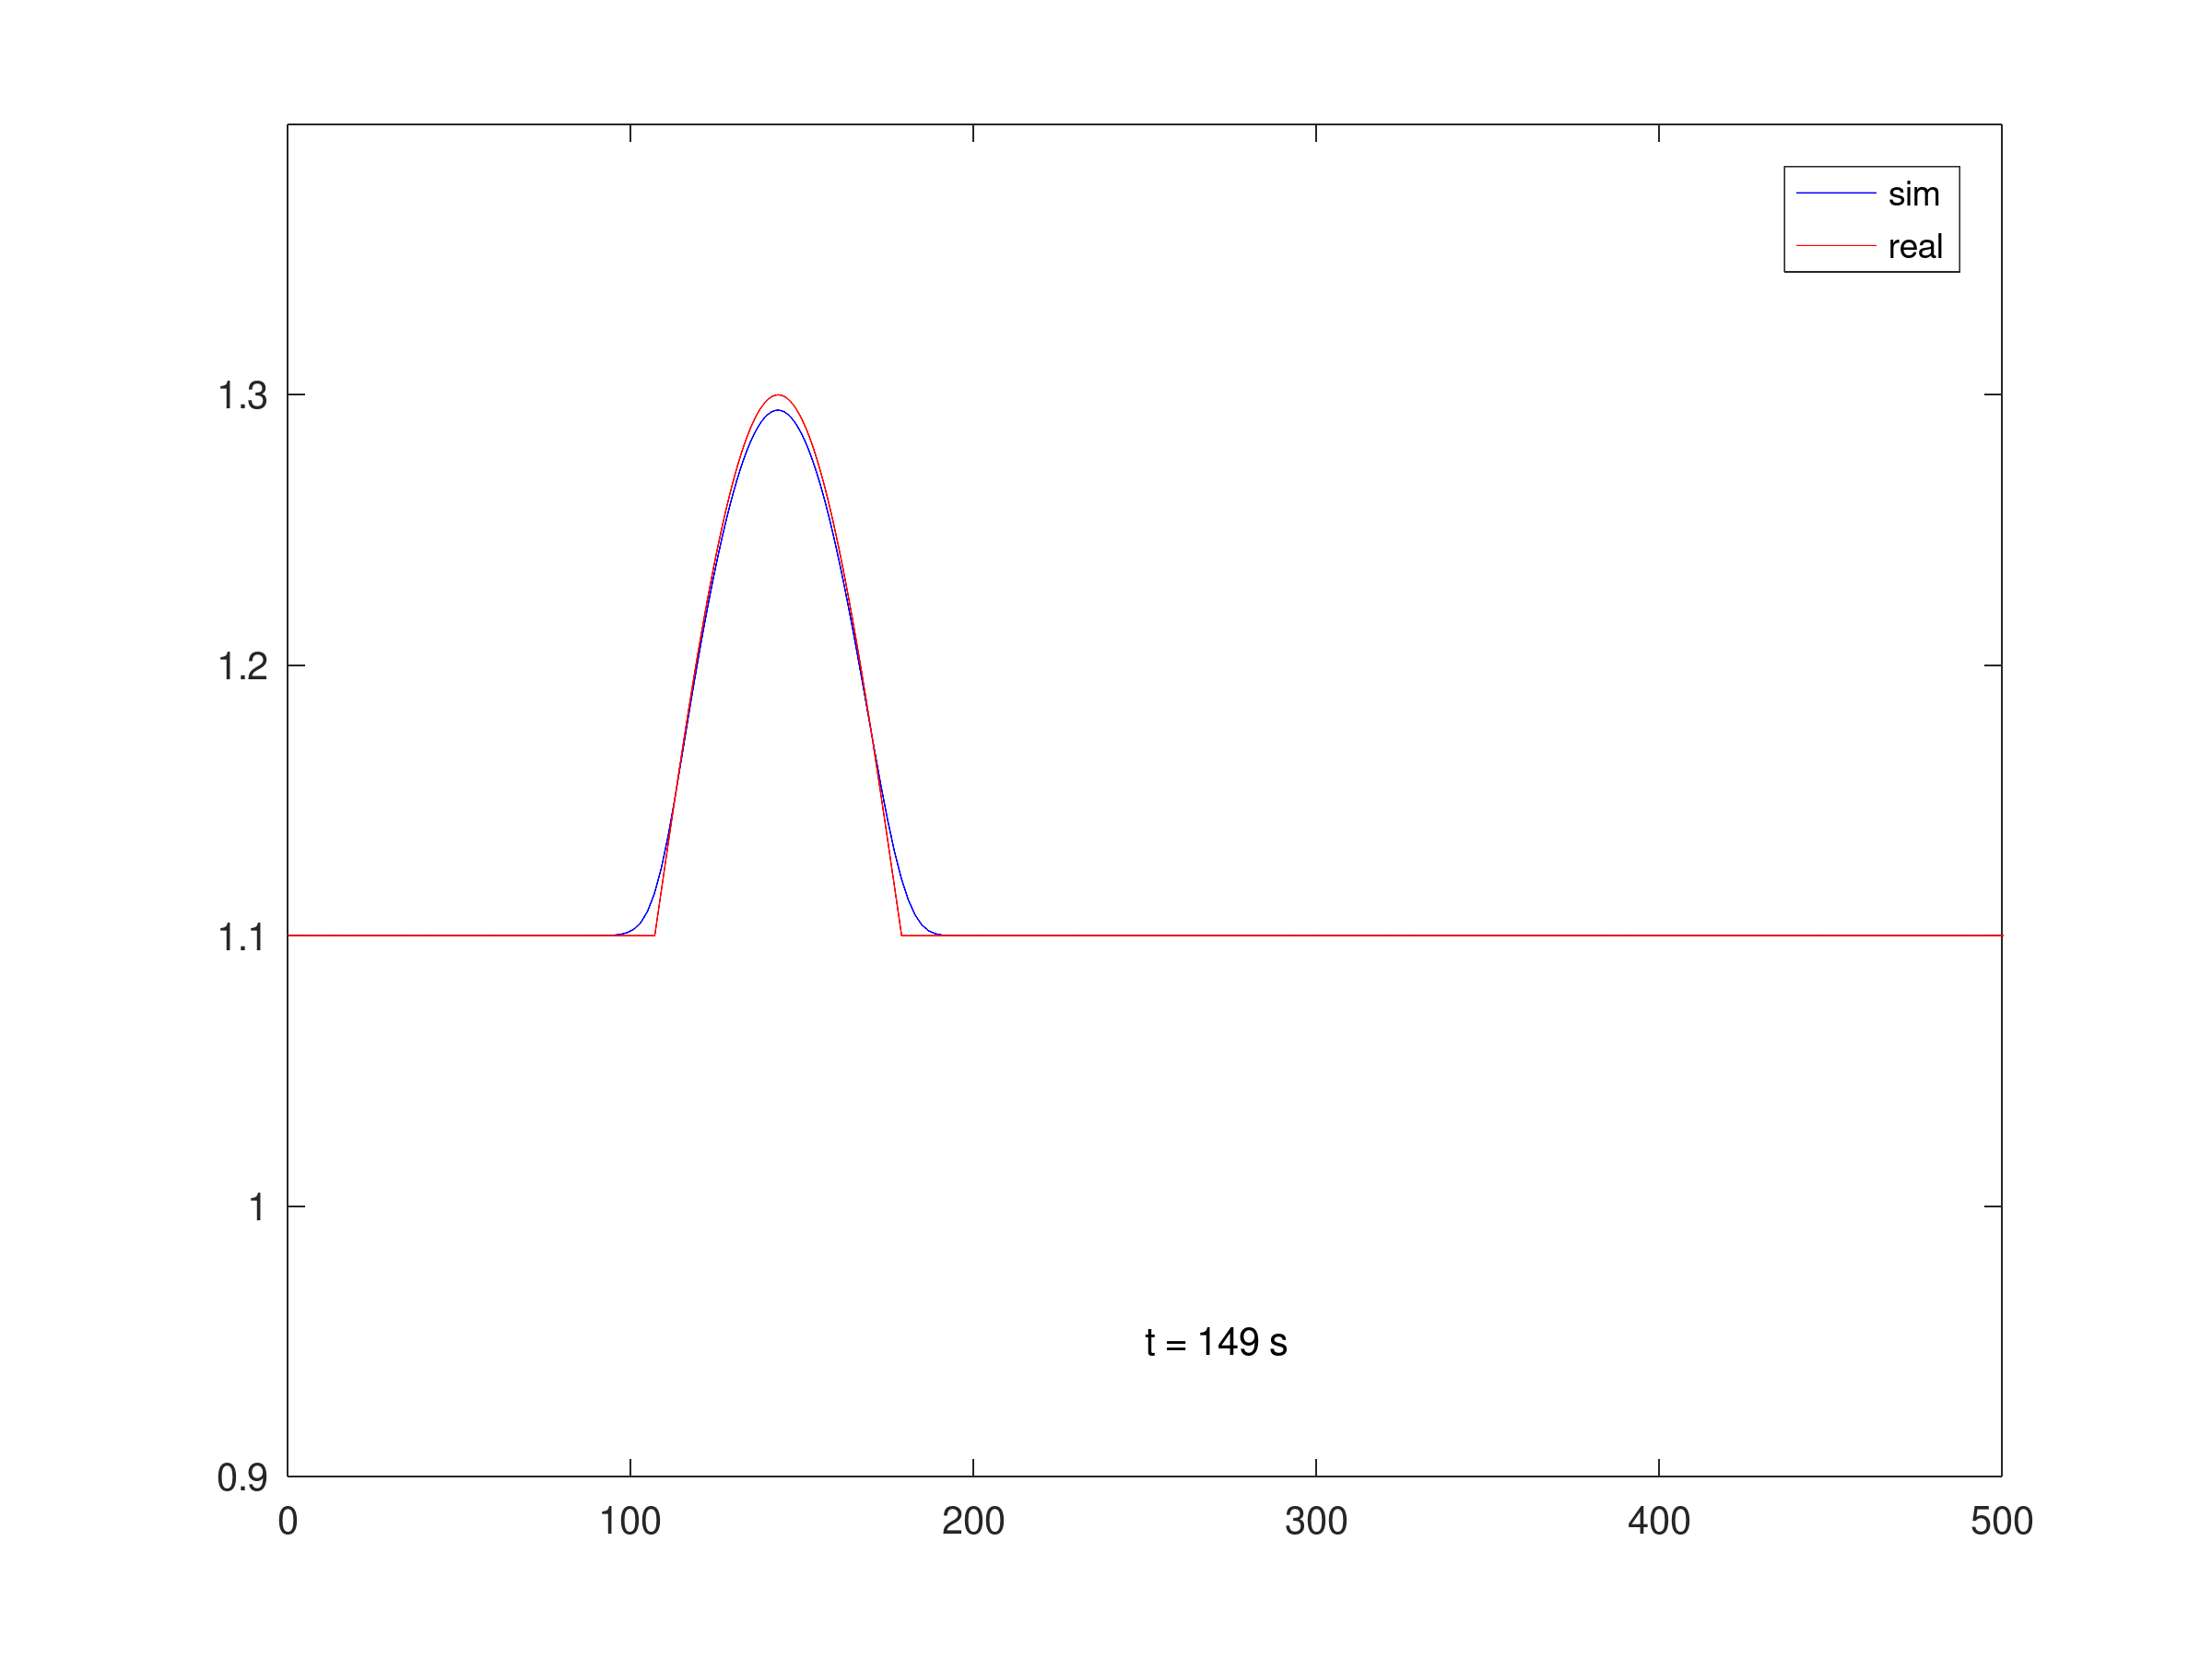
\includegraphics[width=0.8\textwidth]{img/advection.png}
  \end{frame}

%%%%%%%%%%%%%%%%%%%%%%%%%%%%%%%%%%%%%%%%%%%%%%%%%%%%%%%%%%%%%%%%%%%%%%%%%%%%%%%%
% TASK 1 - Setup

\section{Task 1}

  \begin{frame}
    \frametitle{Task 1: Channel simulations - Setup}
    \centering
    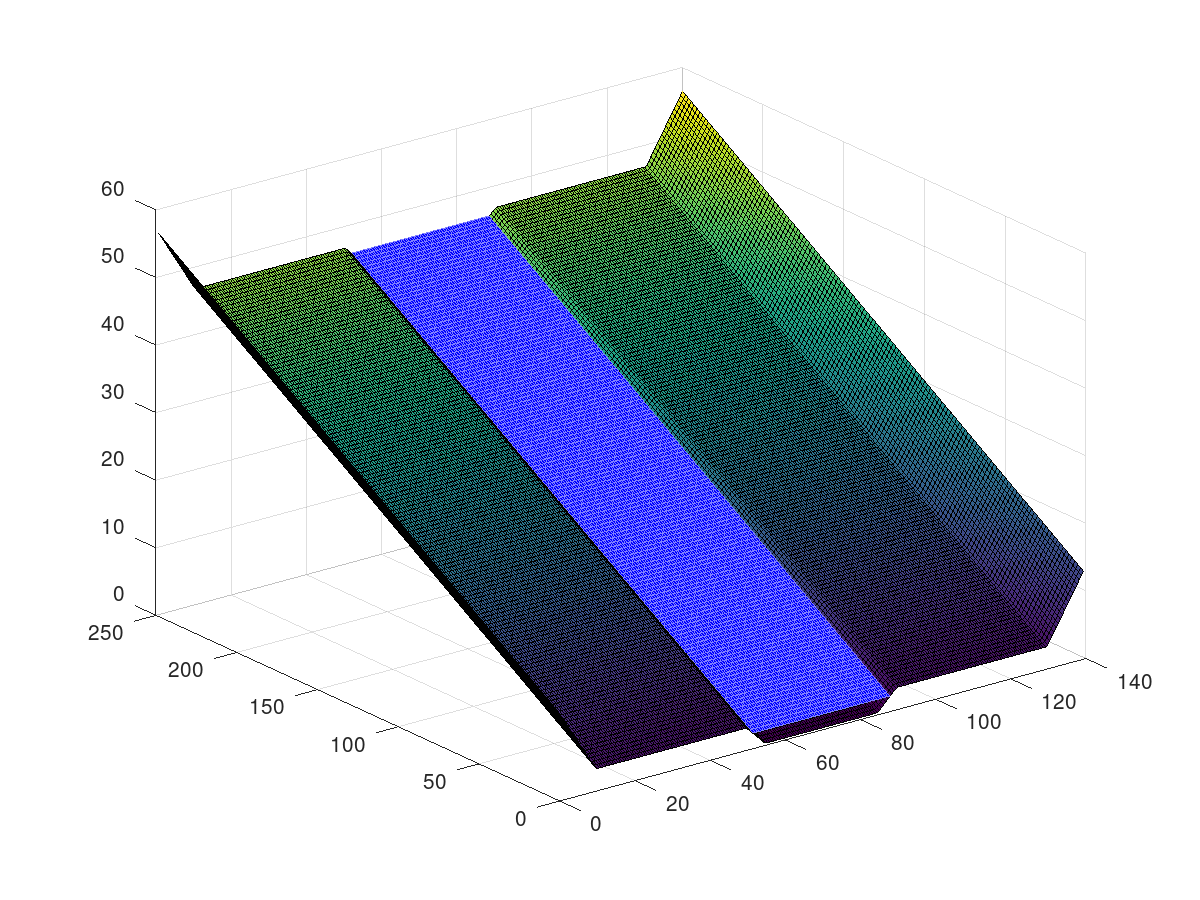
\includegraphics[width=0.6\textwidth]{img/simulation-setup.png}
  \end{frame}

%%%%%%%%%%%%%%%%%%%%%%%%%%%%%%%%%%%%%%%%%%%%%%%%%%%%%%%%%%%%%%%%%%%%%%%%%%%%%%%%
% Animation introduction

\section{Animations}
  {
    \setbeamertemplate{background}{}
    \setbeamercolor{background canvas}{bg=black}
    \setbeamercolor{normal text}{fg=white}
    \usebeamercolor[fg]{normal text}
    \begin{frame}[plain]
      \centering
      \Large{\textbf{Animations:}}\\
      \begin{flushleft}
        \Large{-- Advection simulation}\\
        \Large{-- Constant inflow channel experiment}
      \end{flushleft}
    \end{frame}
  }

%%%%%%%%%%%%%%%%%%%%%%%%%%%%%%%%%%%%%%%%%%%%%%%%%%%%%%%%%%%%%%%%%%%%%%%%%%%%%%%%
% Next Phase

\section{Next Phase}

  \begin{frame}
    \frametitle{Next Phase: 1\textsuperscript{st} emulation step}
    \begin{itemize}
      \item Study effect of variation of one parameter for a specific case study
      \item Run simulations with different parameter values
      \item Generate Input -- Output plot
      \item Interpolate the values to obtain emulator for the chosen parameter
    \end{itemize}
  \end{frame}

\end{document}
